\documentclass[titlepage, a4paper]{article}
\usepackage[english]{babel}
\usepackage[utf8]{inputenc}
\usepackage{graphicx}
\usepackage{color}
\usepackage{mathtools}
\usepackage{float}
\usepackage[parfill]{parskip}
\usepackage[margin=10pt,font=small,labelfont=bf,labelsep=endash]{caption}
\usepackage{epstopdf}
\usepackage{listings}
\epstopdfsetup{suffix=}
\DeclareGraphicsExtensions{.ps}
\DeclareGraphicsRule{.ps}{pdf}{.pdf}{`ps2pdf -dEPSCrop -dNOSAFER #1 \noexpand\OutputFile}

\lstset{literate=%
    {å}{{\r{a}}}1
    {ä}{{\"a}}1
    {ö}{{\"o}}1
    {Å}{{\r{A}}}1
    {Ä}{{\"A}}1
    {Ö}{{\"O}}1
}

\newcommand{\todo}[1] {\textbf{\textcolor{red}{#1}}}

\usepackage{fancyhdr}
\fancyhead[L]{}
\pagestyle{fancy}
\rhead{Alexander Yngve \\ Pål Kastman}
\chead{TDTS08}
\thispagestyle{empty}

\begin{document}

{\ }\vspace{45mm}

\begin{center}
  \Huge \textbf{TDTS08: Lab Report}
\end{center}
\begin{center}
  \Large Lab 2: Instruction Pipelining
\end{center}

\vspace{250pt}

\begin{center}
  \begin{tabular}{|*{3}{p{40mm}|}}
    \hline
    \textbf{Name} & \textbf{PIN} & \textbf{Email} \\ \hline
           {Alexander Yngve} & {930320-6651} & {aleyn573@student.liu.se} \\ \hline
           {Pål Kastman} & {851212-7575} & {palka285@student.liu.se} \\ \hline
  \end{tabular}
\end{center}
\newpage

\tableofcontents
\thispagestyle{empty}
\newpage

\section{Introduction}
The purpose of this lab is to learn how instruction pipelining works and how branch prediction affects the performance of the pipeline.

\section{Pipeline basics I}
\begin{figure}[H]
  \centering
  \begin{tabular}{|c|c|c|c|c|c|}
    \hline
        {IF} & {DA} & {CO} & {FO} & {EX} & {WB} \\ \hline
  \end{tabular}
  \caption{Six stage pipeline.}
  \label{fig:pipeline}
\end{figure}

\section{Pipeline basics II}
When we have a short pipeline we get less time penalty due to that its only one step that needs redoing and therefore its detected earlier. \\

\begin{figure}[H]
  \centering
  \begin{tabular}{|c|c|c|c|c|c|}
    \hline
        {} & {1} & {2} & {3} & {4} & {5} \\ \hline
        {1} & {IF} & {EX} & {} & {} & {} \\ \hline
        {2} & {} & {IF} & {EX} & {} & {} \\ \hline
        {3} & {} & {} & {IF} & {EX} & {} \\ \hline
        {4} & {} & {} & {} & {IF} & {EX} \\ \hline
  \end{tabular}
  \caption{Ideal pipeline operation.}
  \label{fig:ideal_pipe_op}
\end{figure}

\begin{figure}[H]
  \centering
  \begin{tabular}{|c|c|c|c|c|c|c|}
    \hline
        {} & {1} & {2} & {3} & {4} & {5} & {6} \\ \hline
        {1} & {IF} & {EX} & {} & {} & {} & {} \\ \hline
        {2} & {} & {IF} & {EX} & {} & {} & {} \\ \hline
        {25} & {} & {} & {IF} & {} & {} & {} \\ \hline
        {4} & {} & {} & {} & {IF} & {EX} & {} \\ \hline
        {5} & {} & {} & {} & {} & {IF} & {EX} \\ \hline
  \end{tabular}
  \caption{Pipeline operation during conditional jump.}
  \label{fig:condjmp_pipe_op}
\end{figure}

\section{Branch prediction}
Here we analyze how the different branch prediction algorithms perform.

\subsection{Desciption}
For each predictor a benchmark was run according to the following command

$$\text{sim-outorder -bpred \textit{predictor} $\mathtt{\sim}$/TDTS08/bin/go.ss 3 8}$$


\subsection{Solution}
The performance result can be seen in figure \ref{fig:performance} below.

\begin{figure}[H]
	\centering
	\scalebox{0.342}{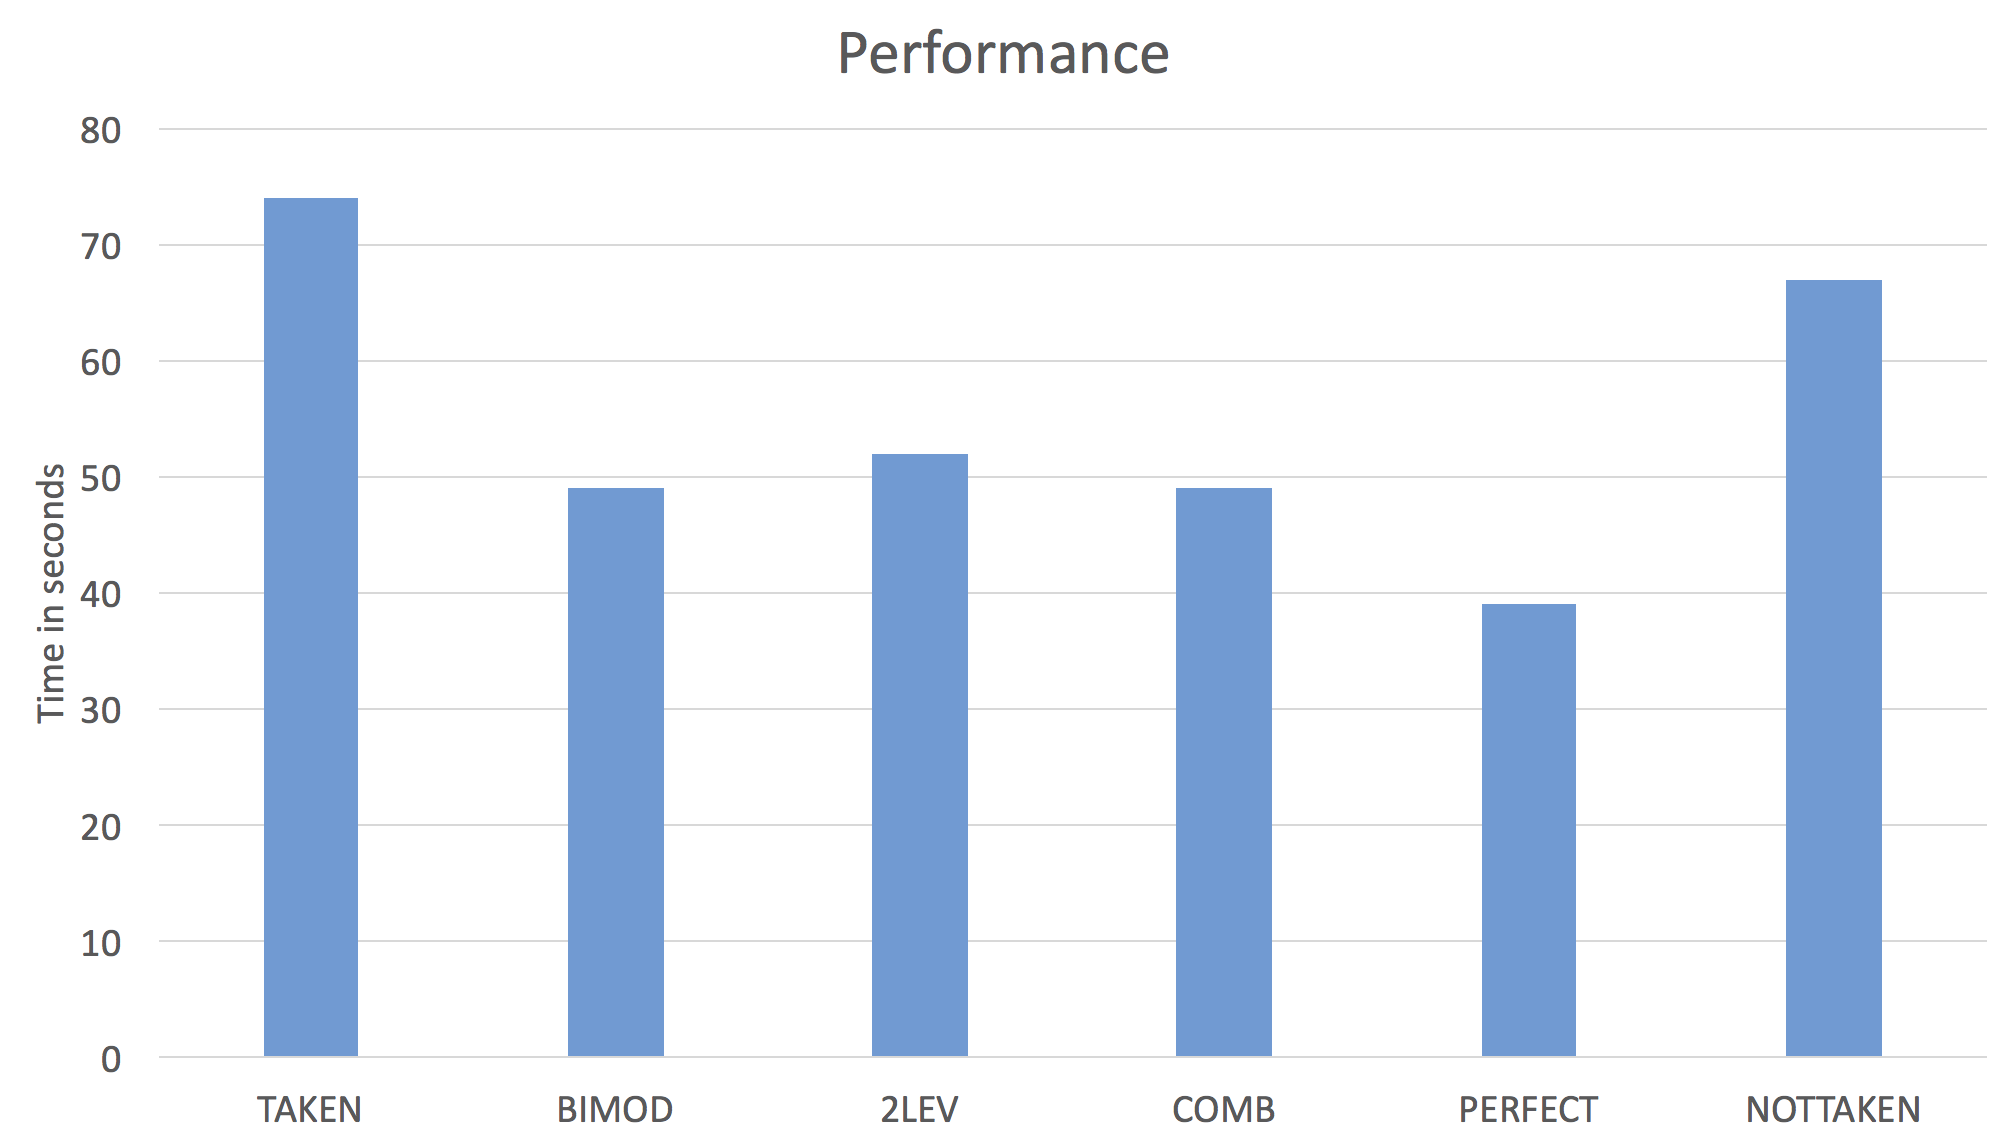
\includegraphics{img/performance.png}}
	\caption{Performance of the different branch prediction algorithms}
	\label{fig:performance}
\end{figure}

\end{document}

